\section{Results}
\subsection{Classification}
The intermediate result after the classification of vegetation is shown in figure~\ref{fig:classification2D}. The accuracy of this classification is presented using a confusion matrix (table~\ref{tab:confusionmatrix}) and the measures for unbalanced datasets in table~\ref{tab:accuracy}.

The ROC-AUC of 0.97 shows the two classes can be separated well, supported by the Matthews correlation coefficient of 0.60, indicating a positive correlation between the predicted and observed classes, and the geometric mean of 0.84. The confusion matrix shows a recall of 0.98 for vegetation and of 0.72 for non-vegetation.

\begin{figure}[!b]
	\centering
	\fbox{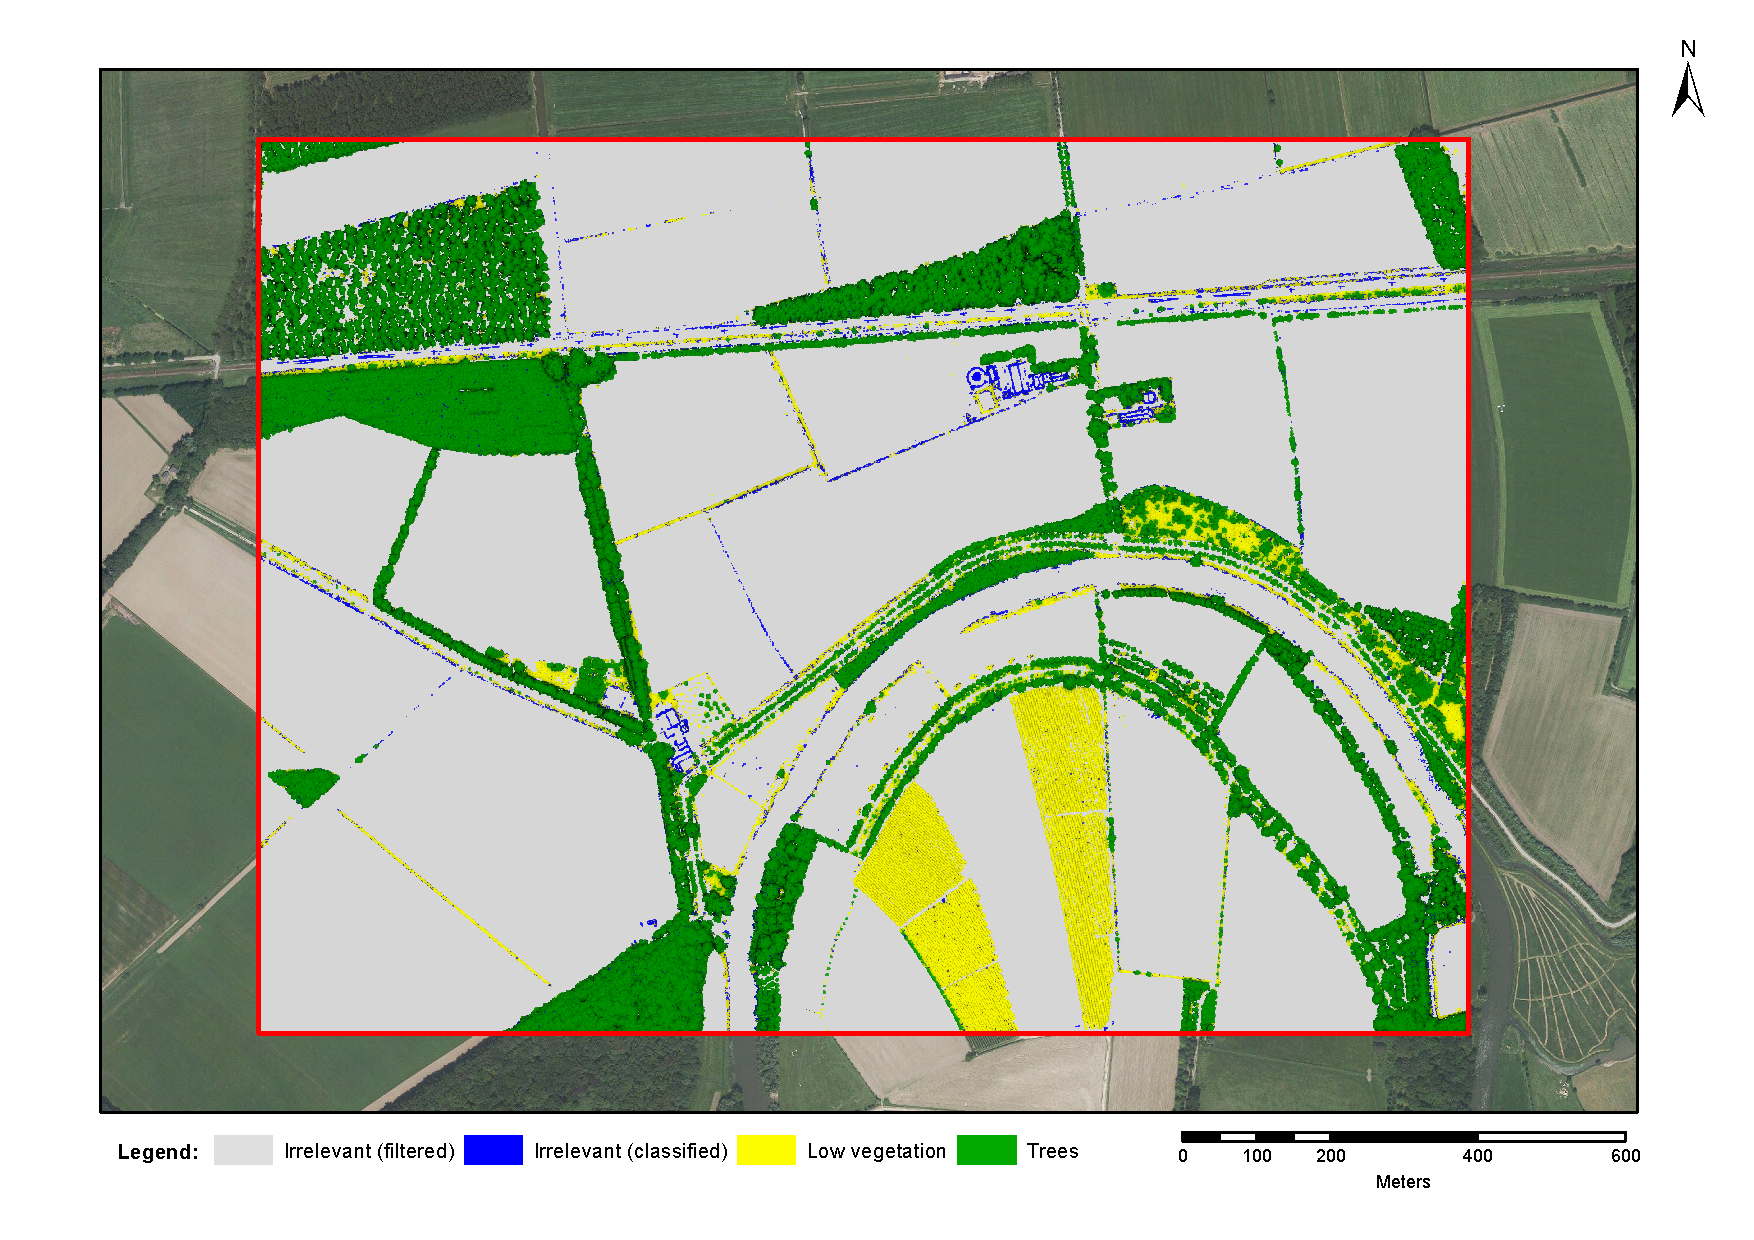
\includegraphics[scale=0.45]{./img/Classification_2D}}
	\caption{A map of the classification results.}
	\label{fig:classification2D}
\end{figure}

\begin{table}
	\caption{A confusion matrix showing the predicted classes against the actual classes of the 10 fold cross-validation accumulated.}
	\label{tab:confusionmatrix}
	\begin{tabular}{ l l l l r}
		\toprule
		\multicolumn{1}{l}{\textbf{Predicted}} & & Vegetation & Irrelevant & Recall\\		
		\midrule
		\textbf{Actual} \\
		Vegetation & & 1159762 & 23438 & 0.98\\
		Irrelevant & & 6416 & 16706 & 0.72\\
		\bottomrule
	\end{tabular}
	\bigskip
	\bigskip
	\caption{Assessment of the accuracy using the average ROC-AUC, MCC and geometric mean of the 10 fold cross-validation.}
	\label{tab:accuracy}
	\begin{tabular}{ l r }
		\toprule
		Metric & Score\\
		\midrule
		ROC-AUC & 0.97 \\
		MCC & 0.60 \\
		Geometric Mean & 0.84 \\
		\bottomrule
	\end{tabular}
\end{table}
\begin{figure}
	\centering
	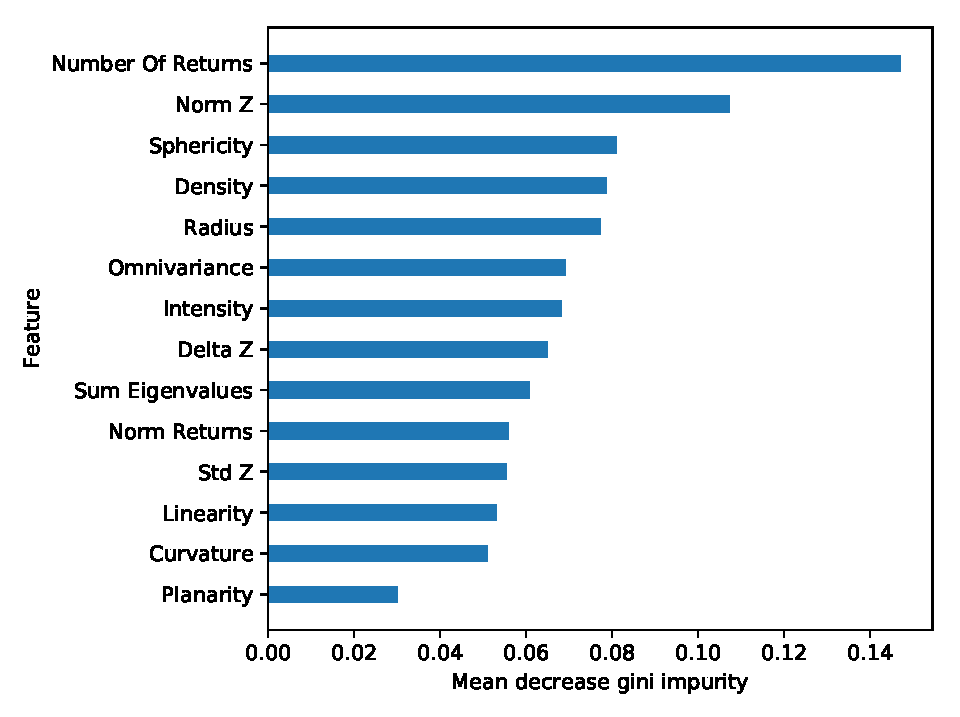
\includegraphics[scale=0.6]{./img/feature_importances}
	\caption{The importance of each feature in the classifier, based on the mean decrease in impurity by the feature. Higher is more important.}
	\label{fig:featureimp}
\end{figure}

The importance of the different features is shown in figure~\ref{fig:featureimp}. It is clear the number of returns is the most important feature when filtering out vegetation. This is not surprising as vegetation is the most prevalent object scanned which produces multiple returns. Not every object with multiple returns is vegetation though (the train power line for example has multiple returns), and not every point with a single return is non-vegetation (especially the edges of low vegetation quite often only have one return). The other features help to further determine to which class a point belongs.

The classification took 1 hour, 6 minutes, and 36 seconds to compute, of which 11m 37s were used for training the classifier, 37m 36s to classify vegetation, and 17m 23s to classify trees and low vegetation. The computation of the features took 1h 25m 34s, of which 17m 34s were used for computing the nearest neighbours and 68m to compute the features.

\subsection{Linear Elements}
To delineate the linear elements first the vegetation points were segmented into rectangular-like objects of which the results are presented in figure~\ref{fig:rect}.

\begin{figure}[!b]
	\centering
	\fbox{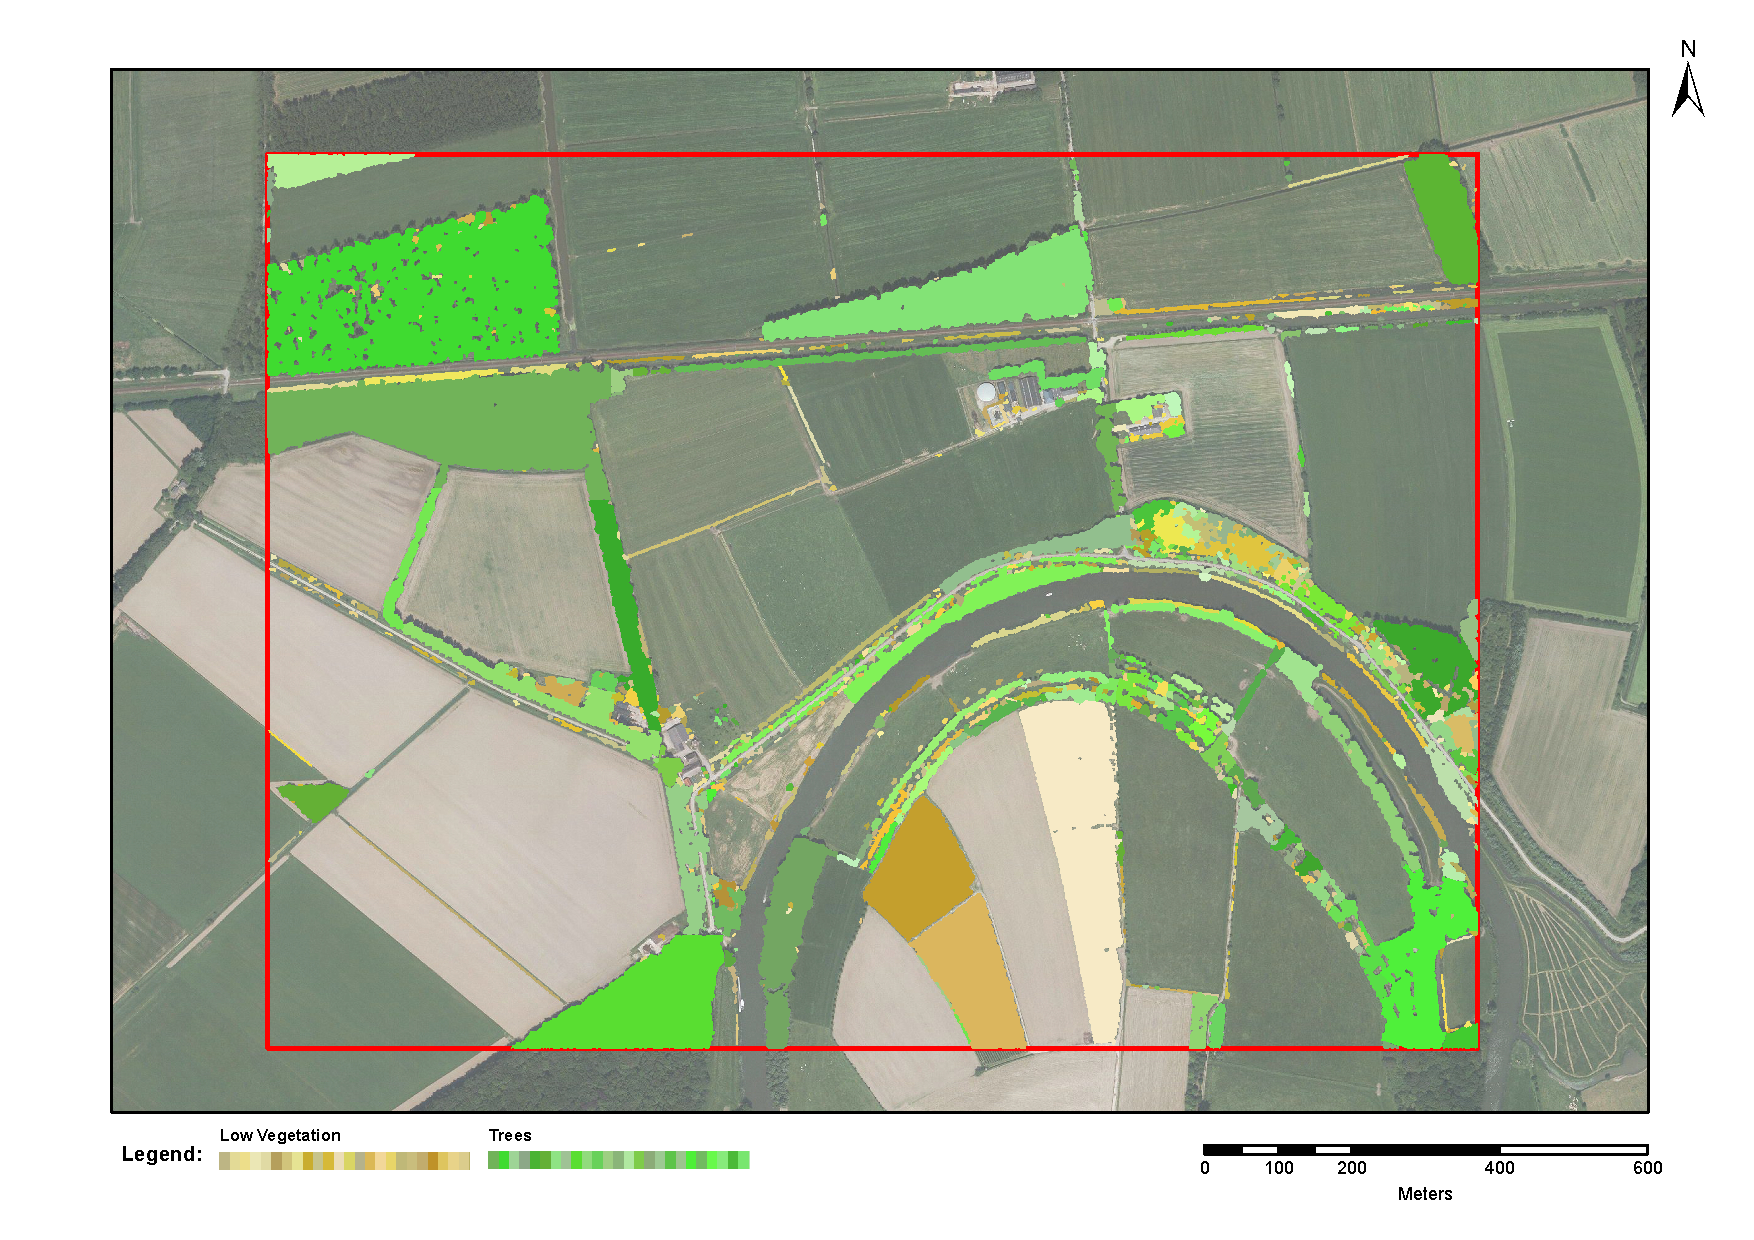
\includegraphics[scale=0.42]{./img/RectObjects}}
	\caption{The resulting rectangular objects.}
	\label{fig:rect}
\end{figure}

The extracted linear objects are shown in figure~\ref{fig:linear}, as well as the result of the manual delineation and the differences between the two. The corresponding confusion matrices are presented in table~\ref{tab:cmtrees} and~\ref{tab:cmlowveg}, with the associated scores shown in table~\ref{tab:linacc}.

The scores are similar for both classes with an overall accuracy of 0.87 for trees and 0.90 for low vegetation, f1 of 0.77 and 0.76, kappa of 0.70 and 0.67, and MCC of 0.70 and 0.67. Although there are errors, the majority of linear elements gets successfully delineated. Especially the areas not belonging to a linear element get separated well, with user's and producer's accuracies of 0.90 and 0.91 for trees, and 0.93 and 0.94 for low vegetation, respectively. The delineation of linear elements is lower at 0.77 and 0.75 for trees, and 0.78 and 0.76 for low vegetation.

The automated process took 4 hours, 47 minutes and 7 seconds to compute for low vegetation, and 1h, 47m and 14s for trees. Since the process was running for trees and low vegetation simultaneously on separate CPU cores the total process took 4h, 47m and 7s.

\begin{figure}
	\centering
	\fbox{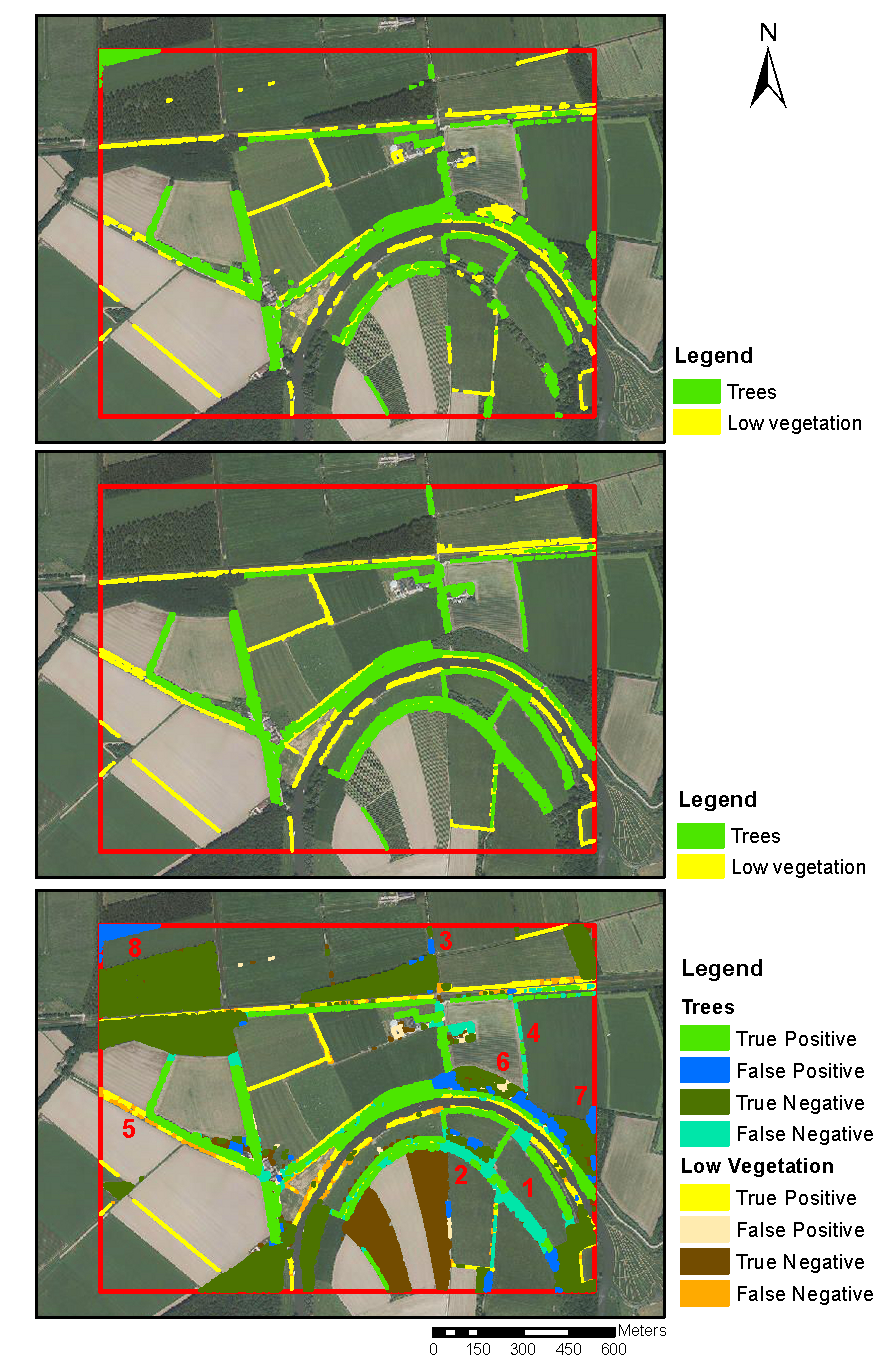
\includegraphics[scale=0.8]{./img/LinCombined}}
	\caption{The result of the delineation of linear objects. Top: automated delineation, middle: manual delineation, bottom: difference between the two.}
	\label{fig:linear}
\end{figure}

%\begin{figure}
%	\centering
%	\fbox{\includegraphics[scale=0.40]{./img/LinObjectsManual}}
%	\caption{Linear vegetation objects determined by manual visual survey.}
%	\label{fig:manual}
%\end{figure}
%
%\begin{figure}
%	\centering
%	\fbox{\includegraphics[scale=0.40]{./img/Difference}}
%	\caption{Differences between the automated and manual delineation.}
%	\label{fig:difference}
%\end{figure}

\begin{table}
	\caption{A confusion matrix showing the automated against the manual delineation for trees in square meters. Overall accuracy shown in the bottom right.}
	\label{tab:cmtrees}
	\begin{tabular}{ l l l l r}
		\toprule
		\multicolumn{1}{l}{\textbf{Automated}} & & Linear & Non-linear & Producer's accuracy\\		
		\midrule
		\textbf{Manual} \\
		Linear & & 70206 & 23188 & 0.75\\
		Non-linear & & 20948 & 226727 & 0.91\\
		User's &&&&\\
		accuracy & & 0.77 & 0.90 & 0.87\\
		\bottomrule
	\end{tabular}
	\bigskip
	\bigskip
	\caption{A confusion matrix showing the automated against the manual delineation for low vegetation in square meters. Overall accuracy shown in the bottom right.}
	\label{tab:cmlowveg}
	\begin{tabular}{ l l l l r}
		\toprule
		\multicolumn{1}{l}{\textbf{Automated}} & & Linear & Non-linear & Producer's accuracy\\		
		\midrule
		\textbf{Manual} \\
		Linear & & 19104 & 6094 & 0.76\\
		Non-linear & & 5243 & 83506 & 0.94\\
%		\midrule
		User's &&&&\\
		accuracy & & 0.78 & 0.93 & 0.90\\
		\bottomrule
	\end{tabular}
	\bigskip
	\bigskip
	\caption{Assessment of the accuracy using the f1, kappa and MCC scores.}
	\label{tab:linacc}
	\begin{tabular}{ l r r}
		\toprule
		Metric & Low vegetation & Trees\\
		\midrule
		f1 & 0.76 & 0.77 \\
		Kappa & 0.67 & 0.70\\
		MCC & 0.67 & 0.70\\
		\bottomrule
	\end{tabular}
\end{table}


% Time to compute

